%% AI4Science 2026 -- conference paper (ACM sigconf)
%% Build:  latexmk -pdf main.tex
%%
%% MODEL IDENTITY: the foundation model evaluated here is TEMPO (Melady/TEMPO,
%% checkpoint TEMPO-80M_v1.pth), loaded by models/tempo_carbon_flux.py and
%% scripts/fine_tune_tempo.py. It is NOT MOMENT. Use "TEMPO" everywhere.
%%
%% Every numeric value in this paper is taken verbatim (or directly derived)
%% from a file in the repository; the source file is noted in a comment beside
%% each table/claim. No numbers were invented.
%%
%% DOUBLE-BLIND: if the AI4Science CFP mandates double-anonymous review, switch
%% \documentclass to [sigconf,anonymous]{acmart} and comment out the author
%% block below before submission. Add author details back only on acceptance.

% \documentclass[manuscript]{acmart}  % single-column review format -- use if CFP requires single-column
\documentclass[sigconf]{acmart}          % NAMED -- use for camera-ready
% \documentclass[sigconf,anonymous]{acmart}   % BLIND -- use for submission
%% =====================================================================
%% AI4Science 2026 -- CONFIGURATION PREAMBLE (preamble.tex)
%% =====================================================================

% --- Core LaTeX Packages ---
\usepackage{booktabs}     % For professional, high-quality table lines
\usepackage{graphicx}     % For including figures and plots
\usepackage{amsmath}      % For advanced math environments and formatting
\usepackage{multirow}    % For multi-row cells inside tables
\usepackage{microtype}   % Enhances line-breaking and stops narrow-column errors

% --- Caption styling: ALL figure/table captions bold TEXT and bold MATH ---
% acmart renders caption text in bold by default, but math ($...$) inside a
% caption does not inherit that weight, so numbers/formulae (R^2, 37--54%, etc.)
% print in normal weight. acmart already loads the caption package, so we declare
% one bold+boldmath caption font and apply it globally to both figure and table
% captions here -- in ONE place, so no per-\caption{} \bfseries/\boldmath prefixes
% are needed anywhere.
\DeclareCaptionFont{bfmath}{\bfseries\boldmath}
\captionsetup{font=bfmath, labelfont=bfmath}

% --- Draft vs. Final Submission Configuration Toggle ---
% Comment out the "DRAFT MODE" block and uncomment the "FINAL SUBMISSION MODE" 
% block when you are ready to generate the camera-ready version for the conference.

%% --- [BLOCK A] DRAFT MODE (Hides copyright & reference blocks to save space) ---
% KEEP printacmref=false until submission: the ACM reference block requires the
% exact rights-form text from ACM's rights-confirmation email, which we do not
% have during drafting. Enabling it now would print placeholder/incorrect rights
% info. The acmart class warns about this by design; the warning is expected.
\settopmatter{printacmref=false}        % Suppresses the ACM reference block
\setcopyright{none}                     % Suppresses copyright statement
\renewcommand\footnotetextcopyrightpermission[1]{} % Clears footer copyright info
%% -------------------------------------------------------------------------------

%% --- [BLOCK B] FINAL SUBMISSION MODE (Uncomment this before final upload) ------
% At submission, replace \setcopyright{...}, \acmDOI and \acmISBN with the exact
% commands supplied in ACM's rights-confirmation email. (Note: acmcopyright is
% deprecated; acmlicensed is the current default.)
% \settopmatter{printacmref=true}       % Restores mandatory ACM reference block
% \setcopyright{acmlicensed}            % replace with the value from the ACM rights email
%% -------------------------------------------------------------------------------

% --- Metadata Settings ---
\acmConference[AI4Science 2026]{Workshop on AI for Science}{2026}{}
\acmYear{2026}
\acmISBN{}
\acmDOI{}

% --- Hyphenation Customizations ---
% Tells LaTeX exactly how to split words unique to your paper if they hit margins
\hyphenation{wet-land eco-sys-tem fore-cast-ing}

\begin{document}

\title{Rethinking Cross-Ecosystem Transfer Learning: Evidence from a
Time-Series Foundation Model for Carbon Flux Forecasting}

%% ---- AUTHOR BLOCK (remove / anonymise for double-blind submission) ----
\author{Paul Ezennolim}
\authornote{Corresponding author.}
\affiliation{%
  \institution{School of Computer Science, University of Sheffield}
  \city{Sheffield}
  \country{United Kingdom}}
\email{tezennolim1@sheffield.ac.uk}

\author{Gaoshan Bi}
\affiliation{%
  \institution{School of Computer Science, University of Sheffield}
  \city{Sheffield}
  \country{United Kingdom}}
\email{gaoshan.bi@sheffield.ac.uk}

\author{Po Yang}
\affiliation{%
  \institution{School of Computer Science, University of Sheffield}
  \city{Sheffield}
  \country{United Kingdom}}
\email{po.yang@sheffield.ac.uk}
%% -----------------------------------------------------------------------

\renewcommand{\shortauthors}{Ezennolim et al.}

\begin{abstract}
Forecasting net ecosystem exchange (NEE) of carbon dioxide underpins
climate modelling and carbon accounting, yet how forecasting models
\emph{transfer across ecosystem boundaries} remains poorly understood.
Classical transfer-learning theory predicts a penalty: a model trained on
one biome should forecast a similar biome better than a dissimilar one.
To investigate how such a model transfers across these boundaries, we compare
TEMPO, a pretrained time-series foundation model, in both zero-shot and
fine-tuned configurations with XGBoost, Random Forest and an LSTM for 96-hour
NEE forecasting across contrasting FLUXNET2015 ecosystems: five wetland
training sites and two held-out test sites, one wetland (UK-AMo, a blanket
bog) and one forest (SE-Htm, a managed spruce forest). The benchmark is our instrument, not our object:
the aim is to characterise the transfer behaviour it reveals. The conventional
models exhibit the expected penalty, degrading by 37--54\% in $R^2$ when
transferring from
the same-ecosystem wetland site to the cross-ecosystem forest site.
TEMPO \emph{inverts} this behaviour: fine-tuned, it attains $R^2=0.728$ on
the cross-ecosystem forest site versus $R^2=0.599$ on the same-ecosystem
wetland site, a $-21.5\%$ ``penalty'', i.e.\ an improvement when crossing
the boundary. All pairwise differences are significant ($p<0.001$, 1000-sample
bootstrap, paired $t$-tests, modified Diebold--Mariano). We attribute the inversion to
alignment between the forest's diurnal dynamics and the
model's pretraining distribution, and we report the result honestly alongside
its central limitation: the baselines use 19 covariates whereas TEMPO is
univariate. The finding suggests that for foundation models, distributional
alignment with pretraining can outweigh nominal domain match.
\end{abstract}

%% CCS concepts: replace with the exact codes/XML pasted from
%% https://dl.acm.org/ccs before submission. The \ccsdesc lines below render
%% without the CCSXML block and are the most likely matches.
\ccsdesc[500]{Computing methodologies~Transfer learning}
\ccsdesc[300]{Computing methodologies~Neural networks}
\ccsdesc[300]{Applied computing~Earth and atmospheric sciences}

\keywords{time-series foundation models, transfer learning, carbon flux,
net ecosystem exchange, FLUXNET, NEE forecasting}

\maketitle

% =====================================================================
\section{Introduction}
% =====================================================================

Net ecosystem exchange (NEE) quantifies the net flux of carbon dioxide
between the terrestrial biosphere and the atmosphere and is a primary
determinant of whether an ecosystem acts as a carbon sink or source.
Reliable short-horizon NEE forecasts support carbon accounting, the design
of monitoring networks, and the assimilation of flux data into Earth-system
models. The FLUXNET2015 network of eddy-covariance towers~\cite{pastorello2020fluxnet2015}
has enabled data-driven NEE modelling at scale, from regression-based
upscaling~\cite{tramontana2016predicting} to global products~\cite{jung2020scaling}.

The stakes are global. The terrestrial biosphere absorbs a large fraction of
anthropogenic carbon-dioxide emissions, and the magnitude and stability of this
land carbon sink remains one of the leading uncertainties in the global carbon
budget~\cite{friedlingstein2023global}. Reducing that uncertainty depends on
dense, well-characterised flux observations and on models that can forecast
fluxes where towers are absent, making the cross-ecosystem behaviour of those
models a question with consequences well beyond any single site.

A persistent obstacle is \emph{transferability}. Flux towers are sparse and
unevenly distributed across biomes, so any operational model must forecast
sites and ecosystems it was not trained on. Classical transfer-learning
theory~\cite{pan2010transfer,weiss2016transfer} predicts a penalty that
grows with the distance between source and target domains: a model trained on
wetlands should forecast an unseen \emph{wetland} better than an unseen
\emph{forest}. Pretrained time-series foundation models~\cite{cao2024tempo}
complicate this picture. Trained on large, heterogeneous corpora, their
cross-domain transfer behaviour in the geosciences, and across ecosystem
boundaries in particular, is essentially unstudied.

This question sits at the intersection of two trends. Foundation models, large
networks pretrained on broad data and adapted to many downstream
tasks~\cite{bommasani2021foundation}, have reshaped language and vision, and
time-series forecasting is the latest domain to follow. In parallel, deep
learning has become central to data-driven Earth-system
science~\cite{reichstein2019deep}. Whether the transfer behaviour that makes
foundation models attractive in those settings carries over to the ecosystem
boundaries of carbon-flux forecasting is precisely what we probe.

This paper asks a single question: \emph{does a time-series foundation model
obey the classical cross-ecosystem transfer penalty in NEE forecasting?}
We find that it does not. Investigating TEMPO alongside XGBoost, Random Forest
and an LSTM on five wetland training sites and two contrasting held-out test
sites, we observe that the conventional models pay the expected penalty
when transferring from a wetland to a forest, whereas the foundation model
\emph{improves} across that same boundary.

\noindent\textbf{Contributions.}
\begin{itemize}
    \item \textbf{First empirical characterisation of cross-ecosystem transfer in a time-series foundation model.} We present, to our knowledge, the first systematic investigation of how a pretrained time-series foundation model transfers across ecosystem boundaries for carbon-flux forecasting.
    
    \item \textbf{Evidence of an inverted cross-\allowbreak ecosystem transfer} to the expectation of classical transfer learning, we observe that the pretrained foundation model achieves higher forecasting accuracy on a cross-ecosystem forest than on a held-out wetland, while conventional machine-learning baselines exhibit the expected degradation.
    
    \item \textbf{Towards understanding transfer behaviour in foundation models.} We analyse the observed inversion and provide evidence that alignment between the target ecosystem dynamics and the model's pretraining distribution may be a stronger determinant of transfer performance than ecosystem similarity alone. We also explicitly discuss the principal limitations of the current study and identify directions for future validation.
\end{itemize}

% =====================================================================
\section{Related Work}
% =====================================================================

\paragraph{Time-series foundation models.}
A recent class of models pretrains a single network on large, diverse
time-series corpora and applies it to unseen series with little or no
task-specific training. TEMPO~\cite{cao2024tempo} is a prompt-based
generative pretrained transformer that decomposes a series into trend,
seasonal and residual components and forecasts them with a GPT-style
backbone. We evaluate the publicly released 80M-parameter checkpoint. Our
focus is not the architecture but its \emph{transfer behaviour} across
ecosystem types, which prior work has not examined for carbon flux.

These models build on a line of specialised deep forecasters, notably
patch-based transformers such as PatchTST~\cite{nie2023patchtst}, which first
showed transformers competing on long-horizon forecasting, and generalise it
by pretraining once across many series rather than fitting each task from
scratch. TEMPO is one of a fast-growing family of such time-series foundation
models. Chronos~\cite{ansari2024chronos} tokenises series and reuses a
language-model
backbone; TimesFM~\cite{das2024timesfm} is a decoder-only forecaster pretrained
on a large temporal corpus; and One Fits All~\cite{zhou2023one} adapts a frozen
pretrained language-model backbone to time series. These share the
pretrain-once, forecast-anywhere premise we test
here; we evaluate TEMPO as a representative instance and leave a multi-model
comparison to future work.

\paragraph{Machine learning for carbon flux.}
Data-driven NEE modelling has a long lineage. Tramontana et
al.~\cite{tramontana2016predicting} benchmark regression algorithms across
global FLUXNET sites; FLUXCOM~\cite{jung2020scaling} upscales fluxes to the
globe; and partitioning methods~\cite{reichstein2005separation} underpin the
NEE products themselves. Tree ensembles such as Random
Forests~\cite{breiman2001random} and gradient boosting~\cite{chen2016xgboost}
remain strong, widely used baselines, with recurrent
networks~\cite{hochreiter1997long} capturing temporal structure.

\paragraph{Transfer learning.}
The classical framing~\cite{pan2010transfer,weiss2016transfer} predicts
that performance degrades as the source and target domains diverge; domain-adaptation
theory makes this precise, bounding target error by source error plus a measure of
divergence between the two domains~\cite{ben2010theory}, and the literature warns
of \emph{negative transfer} when source data harm target performance. Our
contribution is to show that a pretrained foundation model can violate the
first prediction across ecosystem boundaries while the conventional baselines
obey it, and to quantify the negative transfer the baselines suffer.

% =====================================================================
\section{Data and Methods}
% =====================================================================

\subsection{Sites}
We use seven FLUXNET2015 eddy-covariance sites (Table~\ref{tab:sites}),
all distributed under CC-BY-4.0. Five wetland sites form the training pool;
two sites are held out for testing: UK-AMo, a blanket bog, gives a
\emph{wetland-to-wetland} (same-ecosystem) transfer, and SE-Htm, a managed
Norway-spruce forest, gives a \emph{wetland-to-forest} (cross-ecosystem)
transfer. This design isolates the effect of crossing an ecosystem boundary
while holding the training distribution fixed.

% Source: data/metadata/site_characteristics.csv
% TERMINOLOGY NOTE: prose and tables standardise on "wetland" (blanket bog) for
% UK-AMo, per site_characteristics.csv. Some generated figures still label it
% "Peatland" / "Wetland peatland" (e.g. error_analysis, kgml decomposition
% scripts). Decide whether to regenerate those figures for label consistency.
\begin{table}[t]
  \centering
  \caption{FLUXNET2015 sites. Five wetlands are used for training; UK-AMo
  (wetland) and SE-Htm (forest) are held out for testing.}
  \label{tab:sites}
  \small
  \begin{tabular}{@{}llllr@{}}
    \toprule
    Site & Country & Ecosystem & Climate & Records \\
    \midrule
    \multicolumn{5}{@{}l}{\emph{Training (wetland)}}\\
    FI-Lom & Finland & Wetland & Subarctic (Dfc)        & 5\,348 \\
    GL-ZaF & Greenland & Wetland & Tundra (ET)          & 2\,789 \\
    IE-Cra & Ireland & Wetland & Temp.\ oceanic (Cfb)   & 8\,783 \\
    DE-Akm & Germany & Wetland & Temp.\ oceanic (Cfb)   & 3\,836 \\
    FR-LGt & France & Wetland & Temp.\ oceanic (Cfb)    & 5\,294 \\
    \midrule
    \multicolumn{5}{@{}l}{\emph{Test (held out)}}\\
    UK-AMo & U.K. & Wetland & Subpolar oceanic (Cfc)    & 9\,485 \\
    SE-Htm & Sweden & Forest & Temp.\ oceanic (Cfb)     & 5\,437 \\
    \bottomrule
  \end{tabular}
\end{table}

\subsection{Preprocessing}
The FLUXNET2015 data are delivered through the ONEFlux pipeline, in which raw
eddy-covariance fluxes are quality-controlled, $u_*$-filtered and gap-filled
following standardised marginal-distribution-sampling
methods~\cite{papale2006towards}; we use the resulting quality-flagged hourly
product. Half-hourly observations are aggregated to hourly resolution, and a
sliding window maps a 336-hour (two-week) lookback to a 96-hour forecast
horizon. Features are $z$-scored per site using statistics computed within each
split to prevent leakage. The wetland training pool yields $23{,}899$ forecast
sequences. Figure~\ref{fig:neetimeseries} shows the NEE series across all seven
sites, illustrating the contrast between the suppressed wetland fluxes and the
forest's pronounced seasonal--diurnal cycle that the transfer analysis exploits.

% Source: figures/nee_timeseries_all_sites.pdf
\begin{figure*}[t]
  \centering
  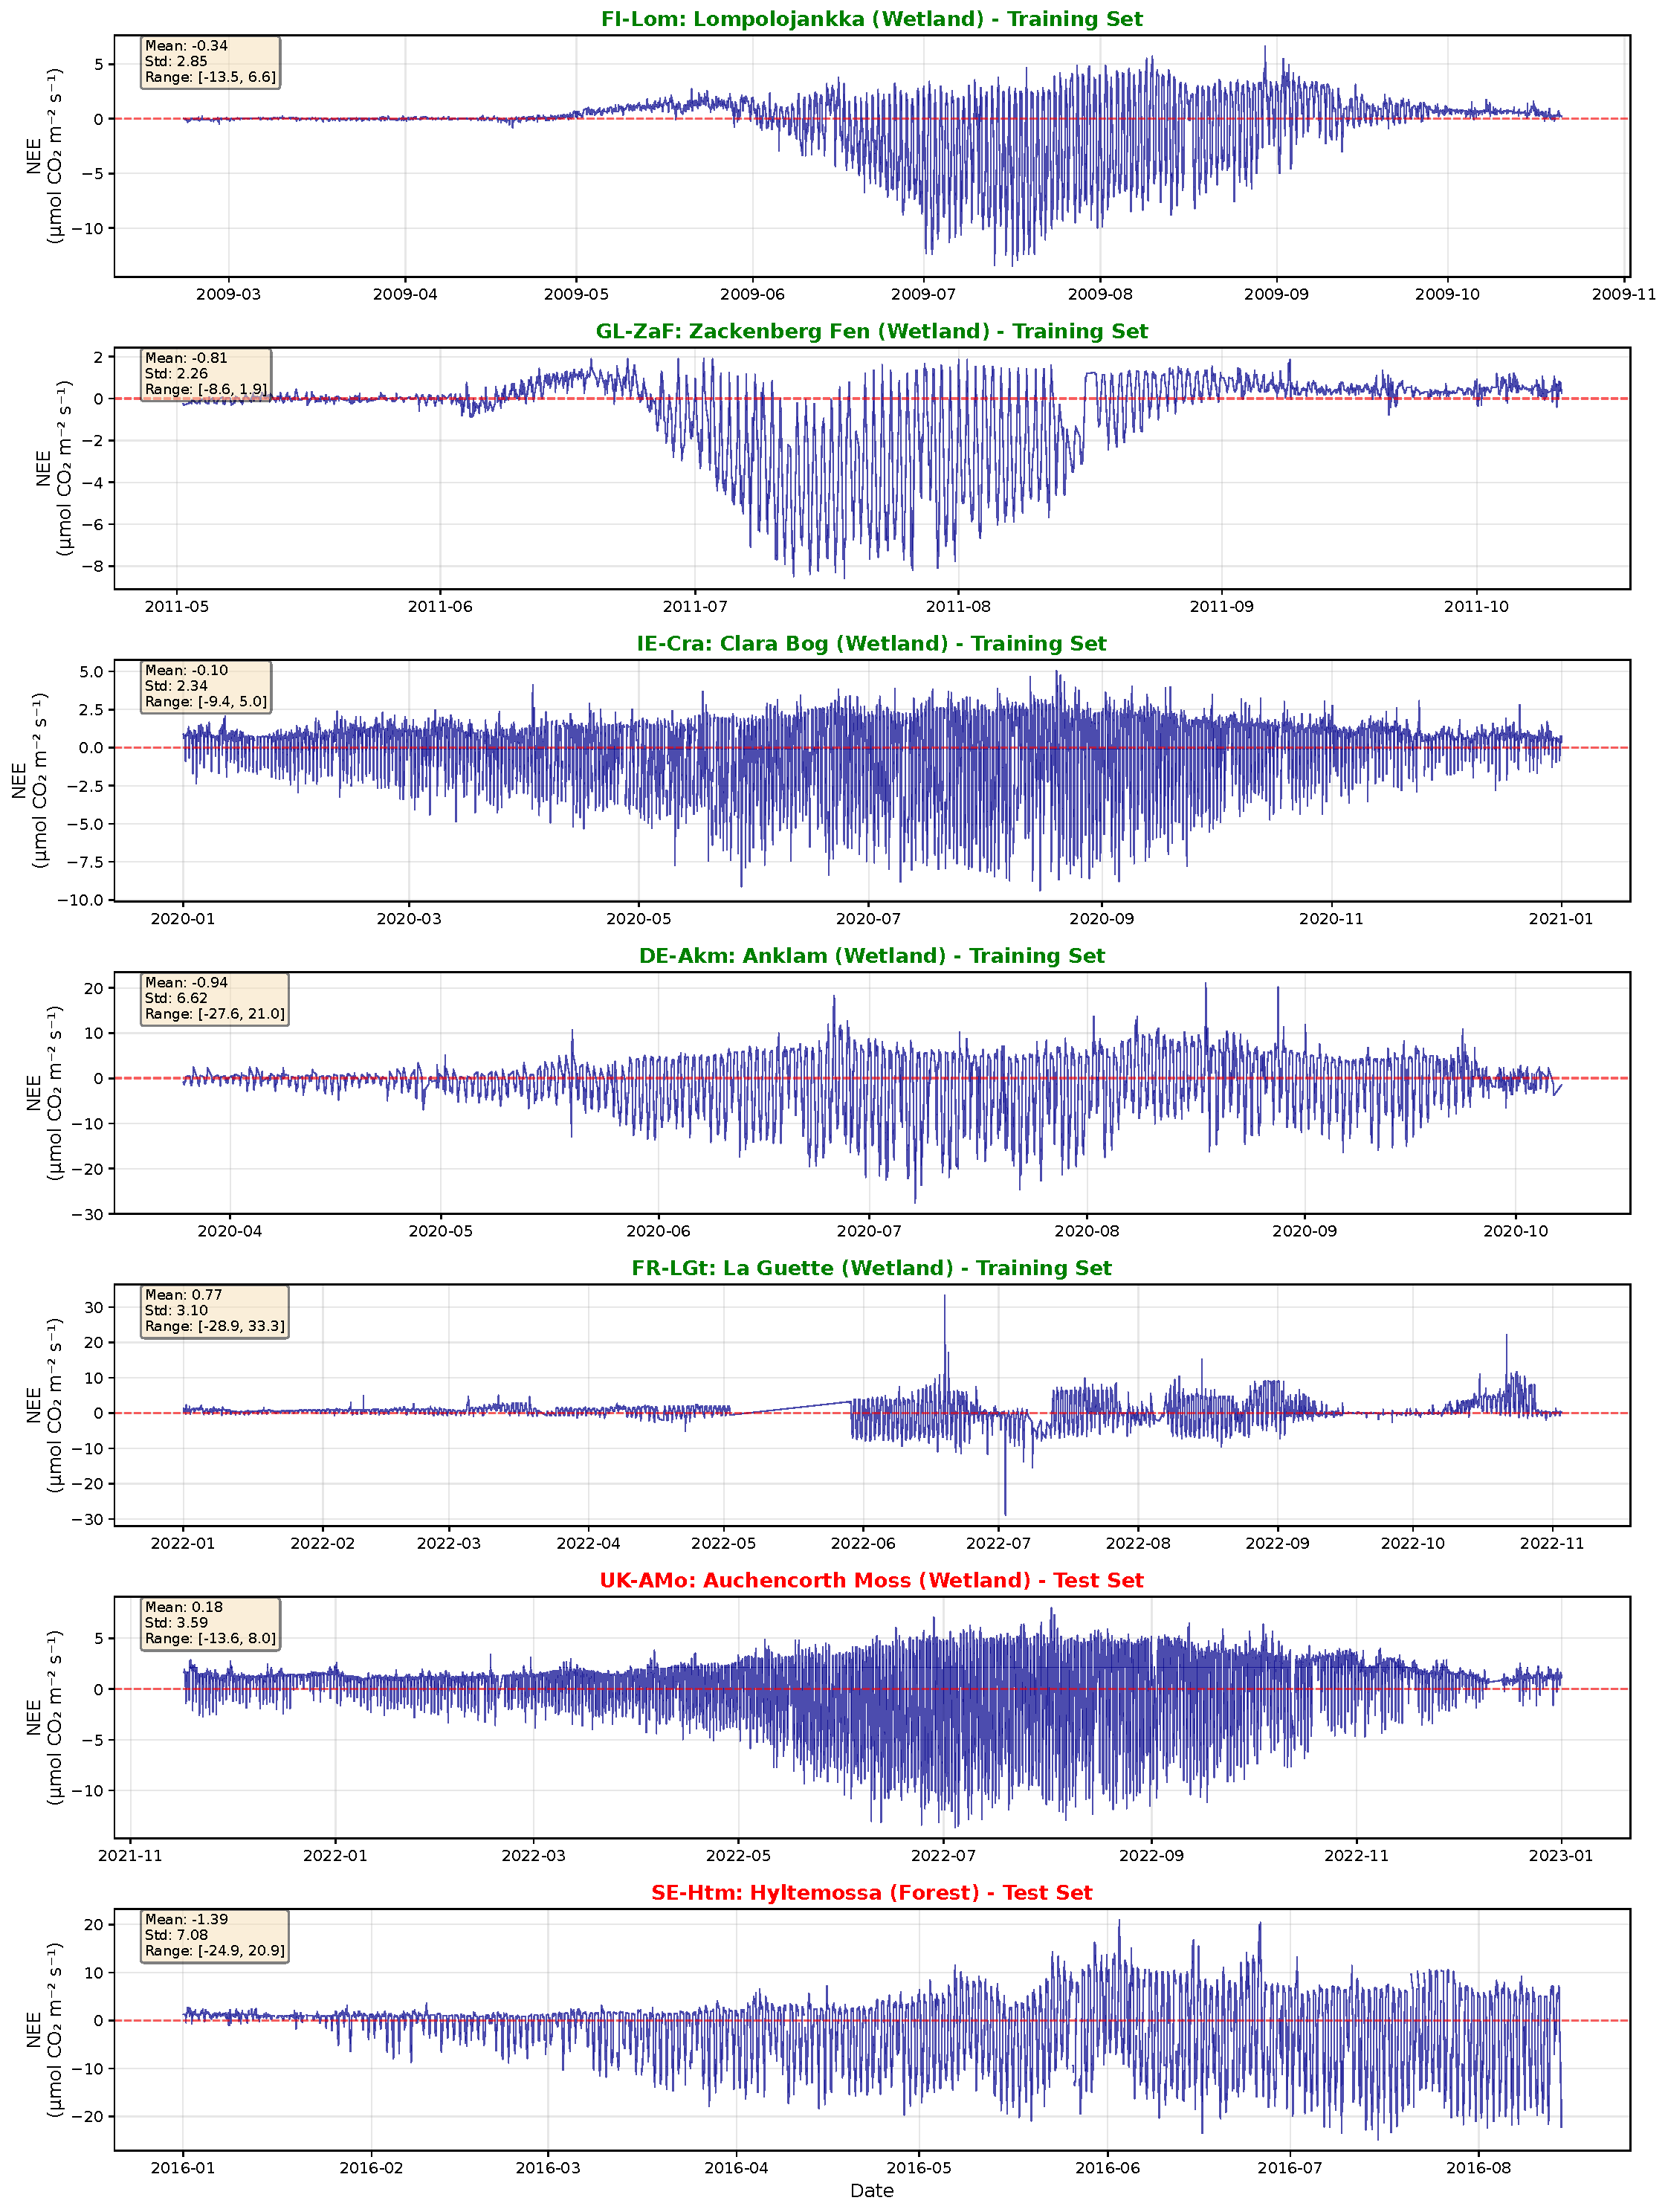
\includegraphics[width=\textwidth]{figures/nee_timeseries_all_sites.pdf}
  \Description{Seven stacked line plots, one per site, showing the half-hourly
  NEE trace over each site's measurement period. The wetland traces hover near
  zero with small fluctuations, while the forest trace swings widely between
  daytime carbon uptake and night-time release.}
  \caption{NEE time series for the five wetland training sites and the two
  held-out test sites (UK-AMo wetland, SE-Htm forest). NEE is in
  $\mu$mol\,CO$_2$\,m$^{-2}$\,s$^{-1}$.}
  \label{fig:neetimeseries}
\end{figure*}

\paragraph{Covariates.}
% Source: scripts/tempo_data_prep.py (build order) and
% scripts/active_learning_analysis.py FEATURE_NAMES (labelled list, 19/timestep):
% SW_IN_F, LW_IN_F, VPD_F, TA_F, PA_F, P_F, WS_F (7 meteorological);
% G_F_MDS, LE_F_MDS, H_F_MDS (3 energy fluxes); MODIS_1..7 (7 bands); DOY, TOD (2 temporal)
The multivariate baselines receive $19$ covariates per timestep, in four groups:
seven meteorological drivers (incoming shortwave radiation, incoming longwave
radiation, vapour-pressure deficit, air temperature, air pressure, precipitation
and wind speed), three surface energy fluxes (ground, latent and sensible heat),
seven MODIS satellite reflectance bands, and two temporal encodings (day-of-year
and time-of-day). TEMPO receives none of these, only the univariate NEE history.

\subsection{Models}
We compare five forecasters under identical windowing:
\begin{itemize}
  \item \textbf{TEMPO (zero-shot)}: The pretrained 80M-parameter checkpoint 
        applied with no downstream task training.
  \item \textbf{TEMPO (fine-tuned)}: The identical checkpoint adapted on the 
        wetland pool via Adam (learning rate: $10^{-4}$; batch size: $32$; 
        up to $50$ epochs with early stopping patience of $10$).
  \item \textbf{XGBoost / Random Forest}: Gradient-boosted and bagged tree 
        ensembles configured with $200$ trees.
  \item \textbf{LSTM}: A two-layer recurrent network utilising $\sim$221k parameters.
\end{itemize}

\paragraph{Information asymmetry (stated openly).}
The comparison is deliberately not matched on inputs. The three baselines are
\emph{multivariate}: they receive $19$ covariates per timestep (meteorological
drivers and satellite indices). TEMPO is \emph{univariate}: it sees only the
NEE target series. This asymmetry favours the baselines on information and is
the principal limitation of the present study; removing it (covariate
conditioning of the foundation model) is the subject of planned follow-up
work. We report results as they stand rather than equalising inputs, and we
return to this point in the discussion.

\subsection{Metrics and statistics}
We report $R^2$, RMSE and MAE on the held-out test sites. Uncertainty is
quantified with 1000-sample bootstrap 95\% confidence intervals; pairwise
model differences are assessed with paired $t$-tests and the modified
Diebold--Mariano test~\cite{harvey1997testing} on 96-hour forecast errors, with
Cohen's $d$ for effect size. All random seeds are fixed at $42$.

% =====================================================================
\section{Results}
% =====================================================================

\subsection{Overall benchmark}
\label{sec:benchmark}
Table~\ref{tab:benchmark} reports the primary benchmark; Figure~\ref{fig:allmodels}
visualises it. On the same-ecosystem wetland site (UK-AMo), the multivariate
baselines are competitive: Random Forest reaches $R^2=0.584$, close to
fine-tuned TEMPO's $R^2=0.599$, with the two separated by a small effect
(Cohen's $d=0.14$ on MAE). On the cross-ecosystem forest site (SE-Htm), the
picture changes sharply: both TEMPO variants exceed $R^2=0.72$ while every
baseline collapses below $R^2=0.28$. All reported pairwise differences are
significant at $p<0.001$.

% Source: results/metrics/all_models_summary.csv (R2, RMSE, MAE)
%         results/analysis/statistical_summary.txt (95% bootstrap CIs on RMSE)
\begin{table}[t]
  \centering
  \caption{Primary 96-hour forecasting benchmark on the two held-out test
  sites. RMSE shown with 1000-sample bootstrap 95\% CI. Lower RMSE/MAE and
  higher $R^2$ are better.}
  \label{tab:benchmark}
  \small
  \begin{tabular}{@{}llccc@{}}
    \toprule
    Site & Model & RMSE (95\% CI) & MAE & $R^2$ \\
    \midrule
    \multirow{5}{*}{UK-AMo}
      & TEMPO Fine-Tuned & 2.318 [2.312, 2.326] & 1.452 & \textbf{0.599} \\
      & Random Forest    & 2.362 [2.357, 2.368] & 1.693 & 0.584 \\
      & XGBoost          & 2.679 [2.674, 2.684] & 2.047 & 0.464 \\
      & TEMPO Zero-Shot  & 2.874 [2.866, 2.882] & 1.754 & 0.384 \\
      & LSTM             & 2.930 [2.923, 2.937] & 1.970 & 0.359 \\
    \midrule
    \multirow{5}{*}{SE-Htm}
      & TEMPO Zero-Shot  & 3.622 [3.611, 3.633] & 2.426 & \textbf{0.752} \\
      & TEMPO Fine-Tuned & 3.794 [3.783, 3.804] & 2.602 & 0.728 \\
      & XGBoost          & 6.178 [6.164, 6.192] & 4.559 & 0.279 \\
      & Random Forest    & 6.212 [6.199, 6.225] & 4.520 & 0.271 \\
      & LSTM             & 6.404 [6.389, 6.418] & 4.638 & 0.225 \\
    \bottomrule
  \end{tabular}
\end{table}

\begin{figure*}[t]
  \centering
  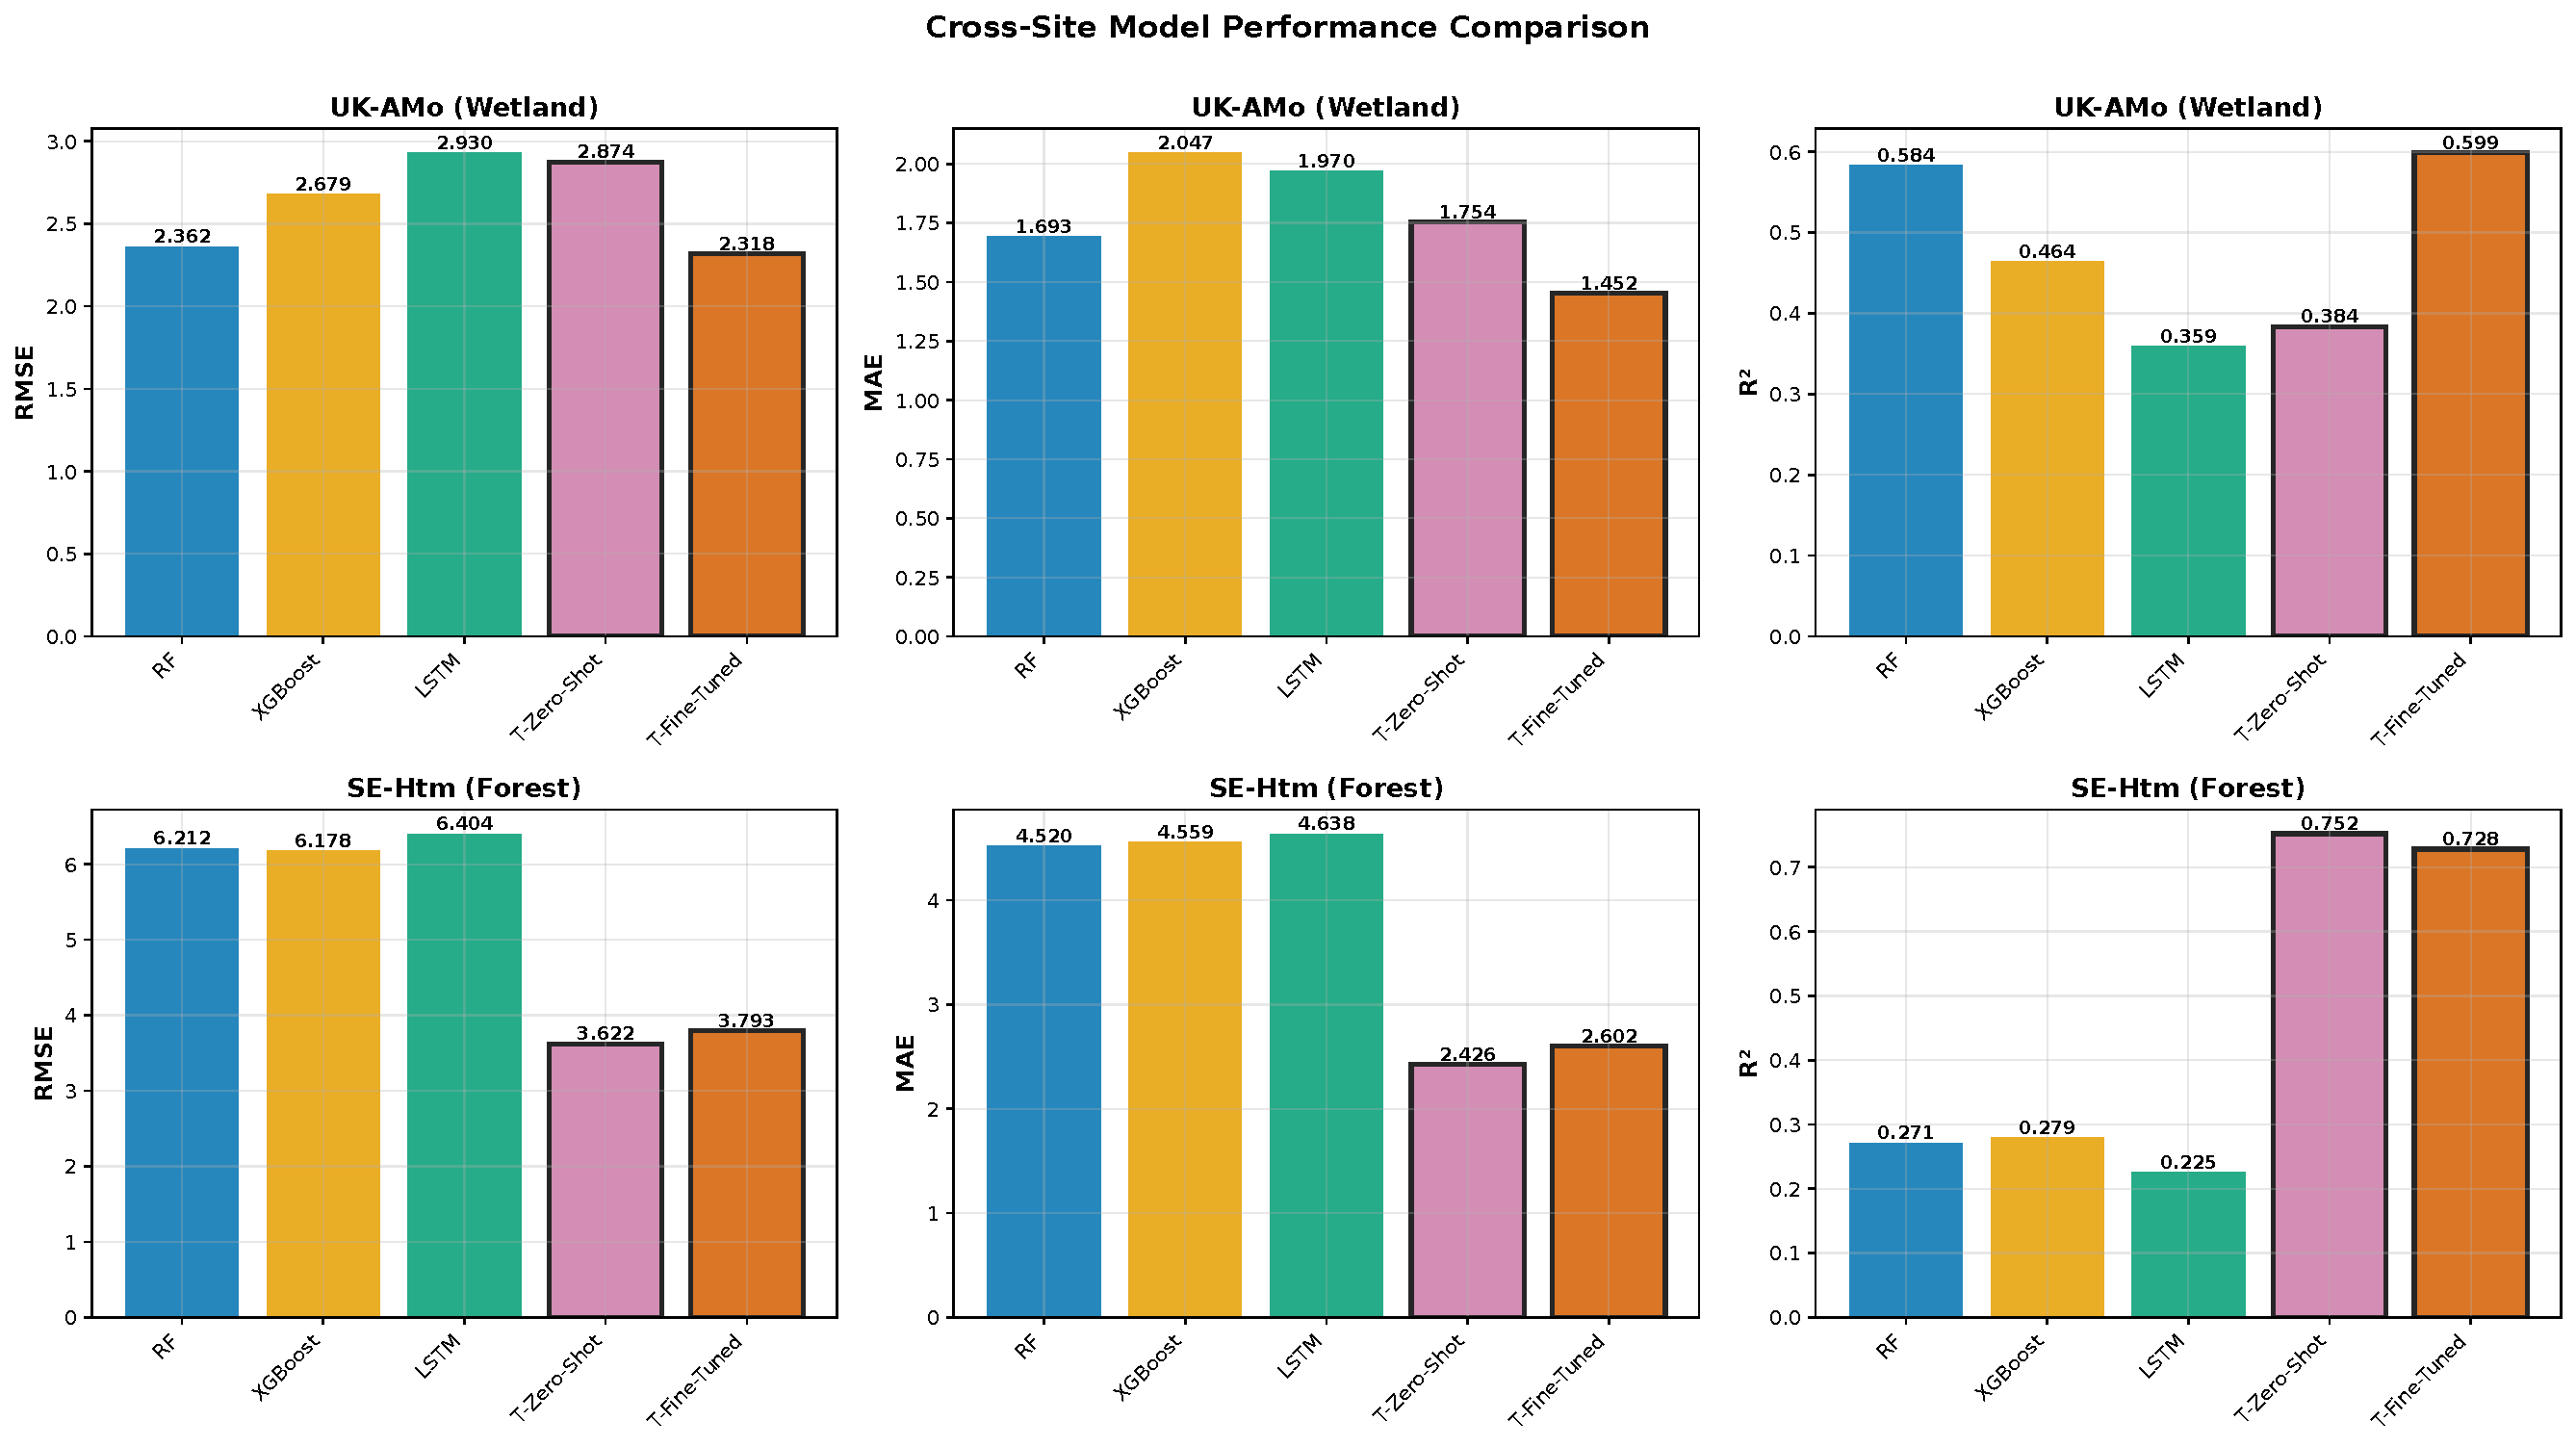
\includegraphics[width=\textwidth]{figures/all_models_comparison.pdf}
  \Description{Grouped bar charts of RMSE, MAE and R-squared for each model at
  each site. On the wetland site the baseline bars sit close to the TEMPO bars,
  but on the forest site the baseline R-squared bars are much shorter than the
  TEMPO bars and their error bars much taller, showing the baselines collapse
  while TEMPO stays accurate.}
  \caption{Model comparison across the two held-out test sites. The baselines
  are competitive on the wetland site but collapse on the forest site, where
  both TEMPO variants remain strong.}
  \label{fig:allmodels}
\end{figure*}

\subsection{The inverted transfer penalty}
\label{sec:inversion}

The headline result is obtained by comparing each model's performance in the
same ecosystem (UK-AMo, wetland) with its performance in a different ecosystem
(SE-Htm, forest). We define the transfer penalty as the relative reduction in
$R^2$ when moving from the wetland to the forest site:
\begin{equation}
\mathrm{penalty}
=
\frac{R^2_{\mathrm{wetland}} - R^2_{\mathrm{forest}}}
     {R^2_{\mathrm{wetland}}},
\label{eq:penalty}
\end{equation}

A positive value corresponds to the expected degradation in performance,
whereas a negative value indicates an inversion. Table~\ref{tab:penalty}
reports these values, computed directly from the benchmark described in
Section~\ref{sec:benchmark}.

% Source: results/metrics/all_models_summary.csv
% Penalty = (R2_wetland - R2_forest)/R2_wetland, computed directly from the
% Table 2 benchmark values so both tables use one consistent harness.
\begin{table}[t]
  \centering
  \caption{Cross-ecosystem transfer penalty (wetland $\rightarrow$ forest),
  computed from the Table~\ref{tab:benchmark} benchmark as
  $(R^2_{\mathrm{wetland}}-R^2_{\mathrm{forest}})/R^2_{\mathrm{wetland}}$.
  Positive $=$ classical degradation; negative $=$ inversion. The three
  baselines degrade by $37$--$54\%$; fine-tuned TEMPO improves by $21.5\%$.}
  \label{tab:penalty}
  \small
  \begin{tabular}{@{}lccc@{}}
    \toprule
    Model & UK-AMo $R^2$ & SE-Htm $R^2$ & Penalty \\
          & (wetland) & (forest) &  \\
    \midrule
    Random Forest    & 0.584 & 0.271 & $+0.313$\ ($+53.6\%$) \\
    XGBoost          & 0.464 & 0.279 & $+0.185$\ ($+39.9\%$) \\
    LSTM             & 0.359 & 0.225 & $+0.134$\ ($+37.3\%$) \\
    \textbf{TEMPO Fine-Tuned} & 0.599 & 0.728 & $\mathbf{-0.129}$\ ($\mathbf{-21.5\%}$) \\
    \bottomrule
  \end{tabular}
\end{table}

Every baseline pays the expected penalty, $+53.6\%$ (Random Forest),
$+39.9\%$ (XGBoost) and $+37.3\%$ (LSTM), losing skill exactly where theory
predicts. Fine-tuned TEMPO does the opposite, recording a $-21.5\%$ penalty:
it is markedly \emph{better} on the cross-ecosystem forest site than on the
same-ecosystem wetland site. On the forest site this lifts fine-tuned TEMPO to
a $+160.9\%$ relative $R^2$ advantage over the best baseline (XGBoost,
$R^2=0.279$), versus a modest $+2.6\%$ over the best baseline (Random Forest)
on the wetland site. The differences are statistically decisive: on
SE-Htm, fine-tuned TEMPO beats XGBoost with $p<0.001$ and a medium effect
(Cohen's $d=0.553$), and the same holds against Random Forest and the LSTM.

% Source: results/metrics/all_models_summary.csv
% TEMPO Zero-Shot:  UK-AMo R2=0.3836, SE-Htm R2=0.7521
% TEMPO Fine-Tuned: UK-AMo R2=0.5988, SE-Htm R2=0.7281
% Zero-shot penalty = (0.384-0.752)/0.384 = -0.958 = -95.8%
The inversion is not an artefact of fine-tuning: it holds for \emph{both}
TEMPO variants, and is in fact larger for the zero-shot model. Zero-shot TEMPO
scores $R^2=0.384$ on the wetland site and $R^2=0.752$ on the forest site, a
penalty of $(0.384-0.752)/0.384 = -95.8\%$, an even stronger inversion than
the fine-tuned model's $-21.5\%$. Fine-tuning on the wetland pool raises the
wetland score ($0.384\rightarrow0.599$) but slightly lowers the forest score
($0.752\rightarrow0.728$). This trade-off is exactly what the alignment
mechanism (Section~\ref{sec:mechanism}) predicts: fine-tuning specialises the
model toward the training biome, helping the in-domain wetland at a small cost
to the out-of-domain forest, yet the forest still wins outright because the
pretrained prior already aligns with its strong diurnal signal.

\subsection{Mechanism}
\label{sec:mechanism}
Why does crossing the boundary \emph{help} the foundation model? The error
distributions (Figure~\ref{fig:errordist}) show that the baselines develop
heavy-tailed, biased errors on the forest site that they do not exhibit on the
wetland site, whereas TEMPO's errors stay comparatively concentrated. We
attribute this to distributional alignment with pretraining. The managed
spruce forest has a large-amplitude diurnal photosynthetic cycle: a strong
periodic signal that stands well clear of the noise floor, of the kind that
dominates the large generic corpora on which foundation models are pretrained.
The wetlands, by contrast, exhibit suppressed flux driven by water-table and
temperature dynamics; their diurnal periodicity, though proportionally
comparable, is small in magnitude and largely buried in noise, leaving a
low-amplitude signal that is comparatively out-of-distribution for a generic
time-series prior. We quantify these signal properties, and report where they
do and do not track forecast skill, in Section~\ref{sec:quantmech}
(Table~\ref{tab:regularity}).
For TEMPO, then, alignment with the pretraining distribution appears to matter
more than nominal ecosystem match; for the covariate-driven baselines, the
forest's NEE dynamics are simply harder to fit from the available drivers.

A complementary ecosystem-prompting experiment supports the alignment view:
fine-tuning TEMPO on forest-aligned data raises forest-site performance to
$R^2=0.766$, a $+5.3\%$ gain over the universal model's $R^2=0.728$,
indicating that the forest signal is not merely easy but specifically
well-matched to what the model represents.

\begin{figure}[t]
  \centering
  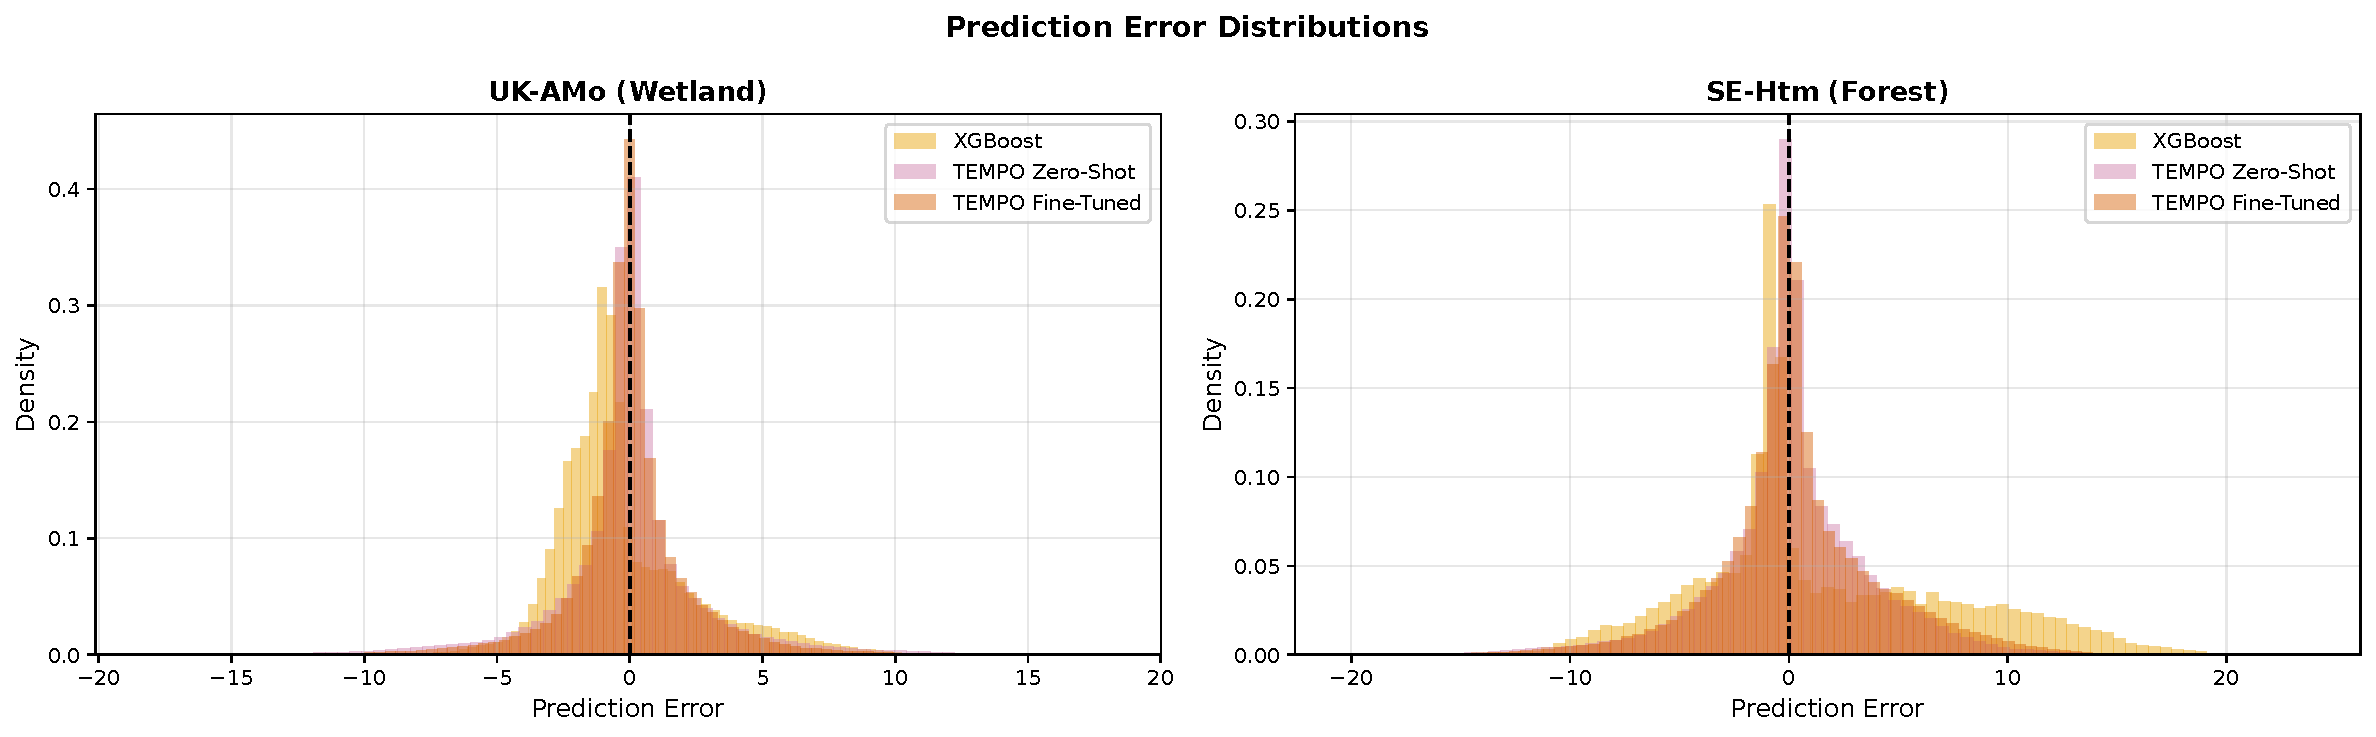
\includegraphics[width=\columnwidth]{figures/tempo_error_distributions.pdf}
  \Description{Two panels of overlaid error-distribution histograms, one per
  test site. The TEMPO histograms form a tall narrow peak centred on zero,
  whereas the baseline histograms are lower, wider and heavy-tailed, indicating
  larger and more frequent extreme errors.}
  \caption{Forecast error distributions for TEMPO on the held-out sites.
  Errors remain concentrated on the forest site, consistent with alignment
  between its strong, large-amplitude diurnal cycle and the model's pretraining
  distribution.}
  \label{fig:errordist}
\end{figure}

% Source: figures/diurnal_patterns_by_ecosystem.png (mean diurnal NEE by ecosystem)
The mean diurnal cycles in Figure~\ref{fig:diurnal} make the alignment argument
concrete: the forest exhibits a pronounced, large-amplitude day--night NEE
oscillation, whereas the wetland's cycle is comparatively flat and small in
amplitude, precisely the distinction between the in-distribution periodic signal
a generic time-series prior forecasts well and the suppressed, out-of-distribution
signal it does not.

\begin{figure}[t]
  \centering
  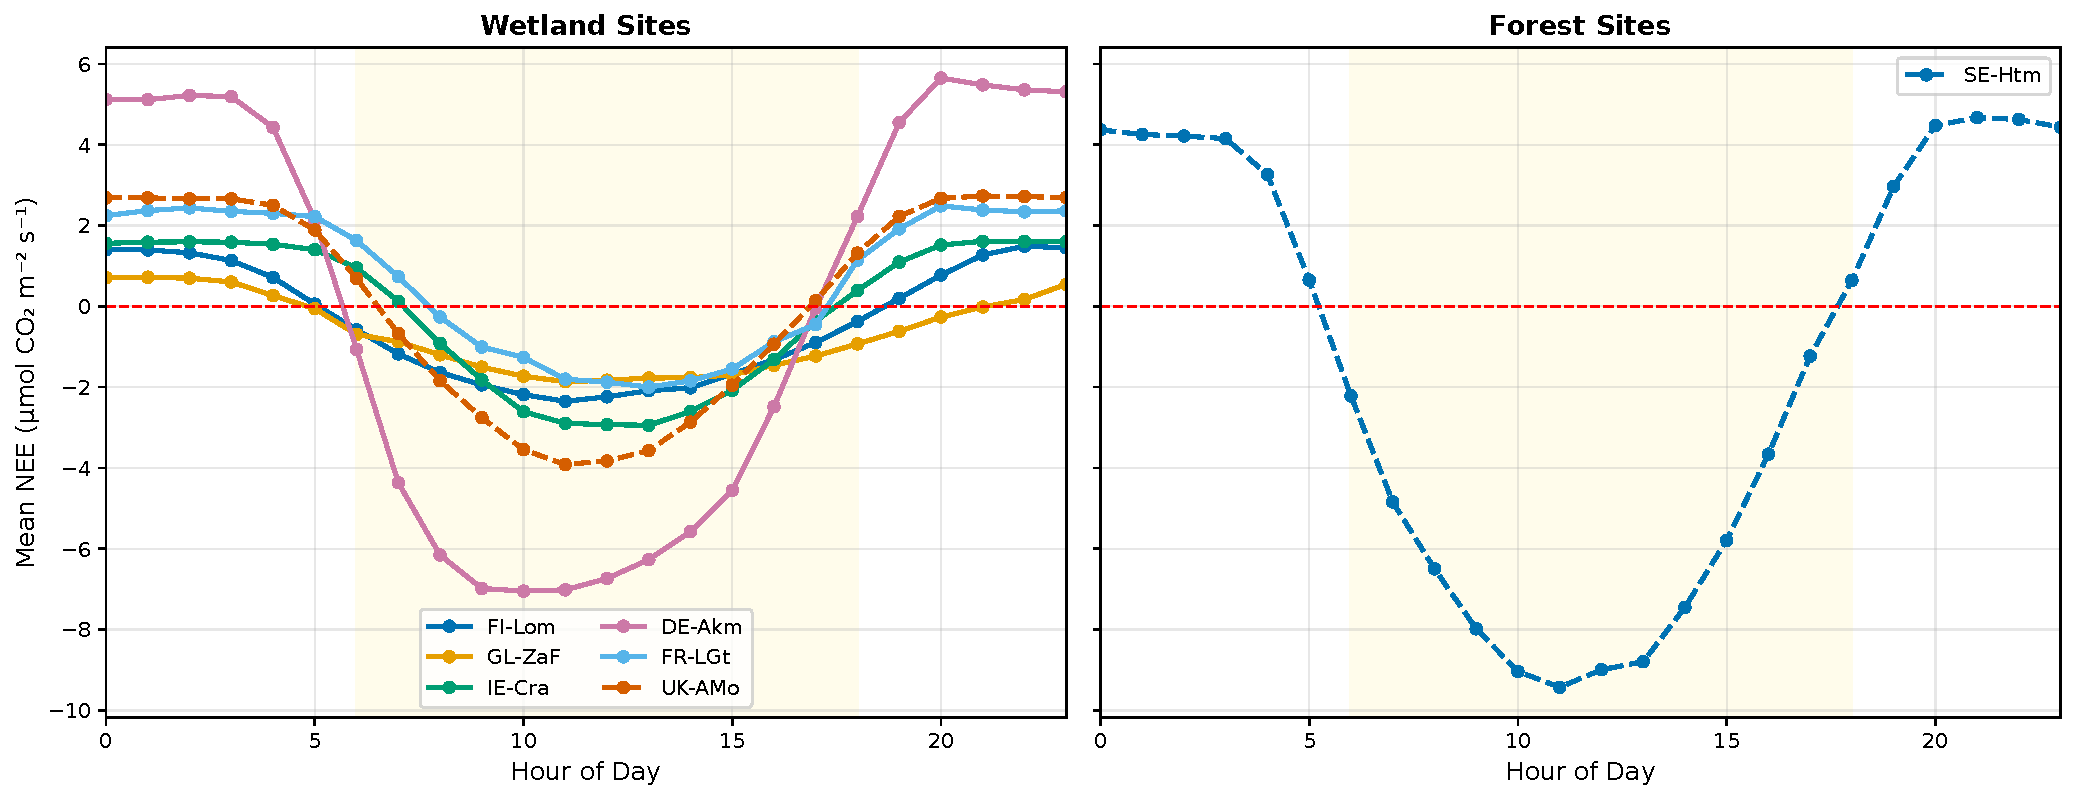
\includegraphics[width=\columnwidth]{figures/diurnal_patterns_by_ecosystem.pdf}
  \Description{Mean NEE plotted against hour of day for each ecosystem. The
  forest curve traces a deep, smooth U-shape with strong daytime uptake and
  night-time release, while the wetland curve stays nearly flat near zero with
  only weak, irregular variation.}
  \caption{Mean diurnal NEE by ecosystem. The forest shows a strong,
  large-amplitude photosynthetic day--night cycle; the wetland's flux is
  suppressed and low in amplitude, consistent with the alignment mechanism for
  the inverted penalty.}
  \label{fig:diurnal}
\end{figure}

\subsection{Quantifying the mechanism: regularity and amplitude}
\label{sec:quantmech}
To test the alignment argument against objective evidence, we compute
signal measures for each site directly from its hourly NEE series, the same
target the models forecast. From each series we estimate the power spectrum with
a Welch periodogram and derive a normalised spectral entropy (lower${}={}$more
regular) and the lag-24\,h autocorrelation (higher${}={}$more diurnally
repeatable); as magnitude-preserving measures we record the absolute spectral
power in the 24-h band and the peak-to-trough amplitude of the mean diurnal
cycle. These measures are summarised in
Table~\ref{tab:regularity}.

The normalised, shape-based measures do \emph{not} explain the inversion. On the
two held-out test sites the forest (SE-Htm) is not more regular than the wetland
(UK-AMo): it has slightly \emph{higher} spectral entropy ($0.388$ vs.\ $0.370$)
and \emph{lower} lag-24\,h autocorrelation ($0.838$ vs.\ $0.867$), yet is
forecast far better (zero-shot $R^2=0.752$ vs.\ $0.384$). A ``more regular
signal, better forecast'' account is therefore not supported by these data.

The amplitude measures, by contrast, order the two sites as $R^2$ does. The
forest's diurnal signal is several times larger than the wetland's, absolute
24-h spectral power $25.9$ vs.\ $6.7$, and peak-to-trough diurnal amplitude
$14.0$ vs.\ $6.5$ (Table~\ref{tab:regularity}), consistent with an amplitude /
signal-to-noise reading of the mechanism rather than a regularity one.

Three caveats bound this. First, per-site zero-shot $R^2$ is available for only
the two test sites, so this is a two-site \emph{ordering}, not a correlation
across sites. Second, amplitude is not strictly an ecosystem property: the
wetland DE-Akm has the second-largest diurnal amplitude of the seven sites.
Third, three sites (GL-ZaF, FR-LGt, DE-Akm) required substantial gap-filling, so
their reported amplitudes are lower-bound estimates.

\begin{table}[t]
  \centering
  \caption{Objective signal measures per site, computed from each site's hourly
  NEE series (Welch periodogram; normalised spectral entropy, lower${}={}$more
  regular; peak-to-trough diurnal amplitude; absolute 24-h spectral power).
  Zero-shot TEMPO $R^2$ is available only for the two held-out test sites
  (dash otherwise).}
  \label{tab:regularity}
  \Description{Table of seven flux sites listing spectral entropy, diurnal
  amplitude and absolute 24-hour spectral power computed from each site's NEE
  series. The forest site SE-Htm has the largest diurnal amplitude and 24-hour
  power but not the lowest spectral entropy, and the wetland DE-Akm has the
  second-largest amplitude. Zero-shot R-squared is shown only for the two test
  sites, UK-AMo (0.384) and SE-Htm (0.752).}
  \small
  \setlength{\tabcolsep}{4.5pt}
  \begin{tabular}{@{}llrrrr@{}}
    \toprule
    Site & Ecosystem & \shortstack[r]{Spec.\\entropy} &
    \shortstack[r]{Diurnal\\amp.} & \shortstack[r]{Abs.\ 24-h\\power} &
    \shortstack[r]{Zero-shot\\$R^2$} \\
    \midrule
    \multicolumn{6}{@{}l}{\emph{Training (wetland)}}\\
    FI-Lom            & Wetland & $0.404$ & $3.5$  & $3.9$  & --- \\
    GL-ZaF$^{\dagger}$ & Wetland & $0.373$ & $2.2$  & $2.0$  & --- \\
    IE-Cra            & Wetland & $0.419$ & $4.5$  & $2.7$  & --- \\
    DE-Akm$^{\dagger}$ & Wetland & $0.432$ & $11.0$ & $17.7$ & --- \\
    FR-LGt$^{\dagger}$ & Wetland & $0.535$ & $3.5$  & $2.9$  & --- \\
    \midrule
    \multicolumn{6}{@{}l}{\emph{Test (held out)}}\\
    UK-AMo            & Wetland & $0.370$ & $6.5$  & $6.7$  & $0.384$ \\
    SE-Htm            & Forest  & $0.388$ & $14.0$ & $25.9$ & $0.752$ \\
    \bottomrule
  \end{tabular}
  \par\smallskip
  {\footnotesize $^{\dagger}$Substantial gap-filling ($19$--$28\%$ missing before
  fill); reported diurnal amplitude and 24-h power are lower-bound estimates.}
\end{table}

\subsection{Error structure}
\label{sec:errorstructure}
% Source: figures/error_analysis/error_by_hour_{SE-Htm,UK-AMo}.pdf
Resolving forecast error by hour of day sharpens the mechanism
(Figure~\ref{fig:errorhour}). On the forest site the error follows a clean,
regular diurnal profile that mirrors the photosynthetic cycle, exactly the
kind of large-amplitude, high-SNR periodic signal the pretrained model
represents well, so the foundation model tracks it with low, predictable error
throughout the day. On the wetland
site the hourly error is flatter and noisier, lacking the strong diurnal
signature, consistent with a suppressed, small-amplitude flux that is harder to
anticipate from a generic temporal prior. The contrast in error structure thus
echoes the alignment argument: the forest's large, clean diurnal amplitude is
what the model tracks, the magnitude of its periodic flux being central to the
alignment rather than incidental to it.

\begin{figure}[t]
  \centering
  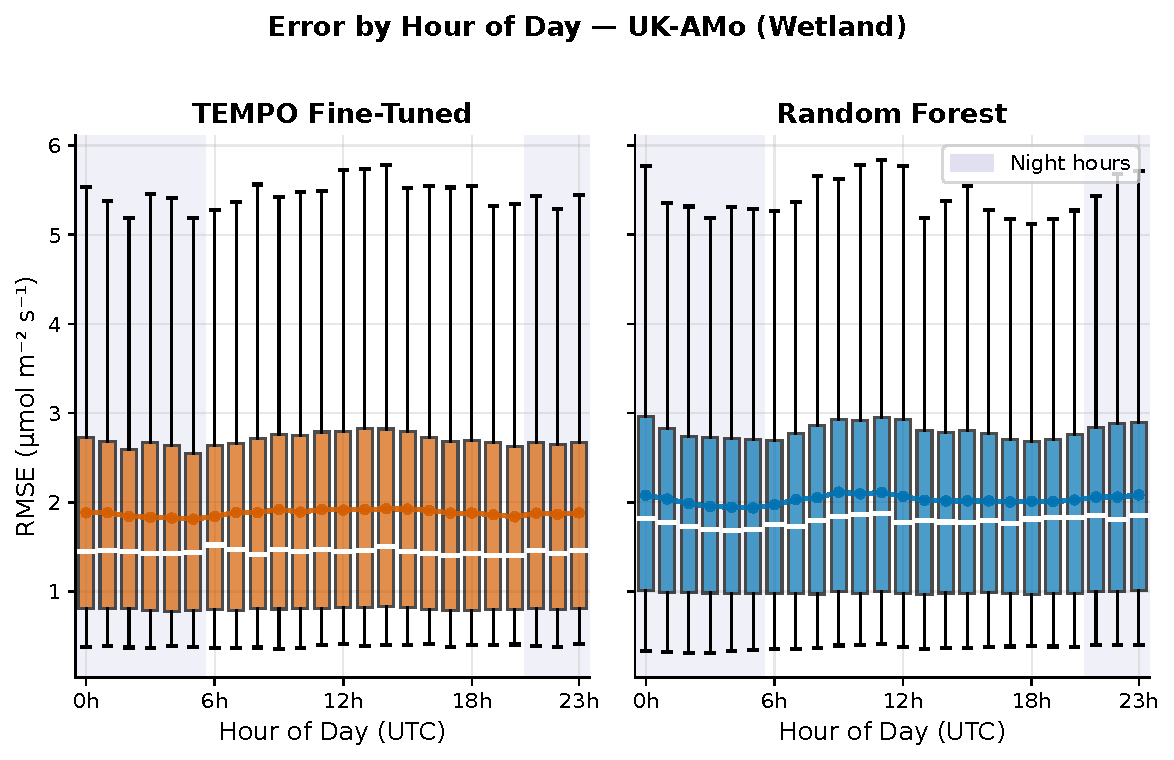
\includegraphics[width=0.95\columnwidth]{figures/error_by_hour_UK-AMo.pdf}
  \\
  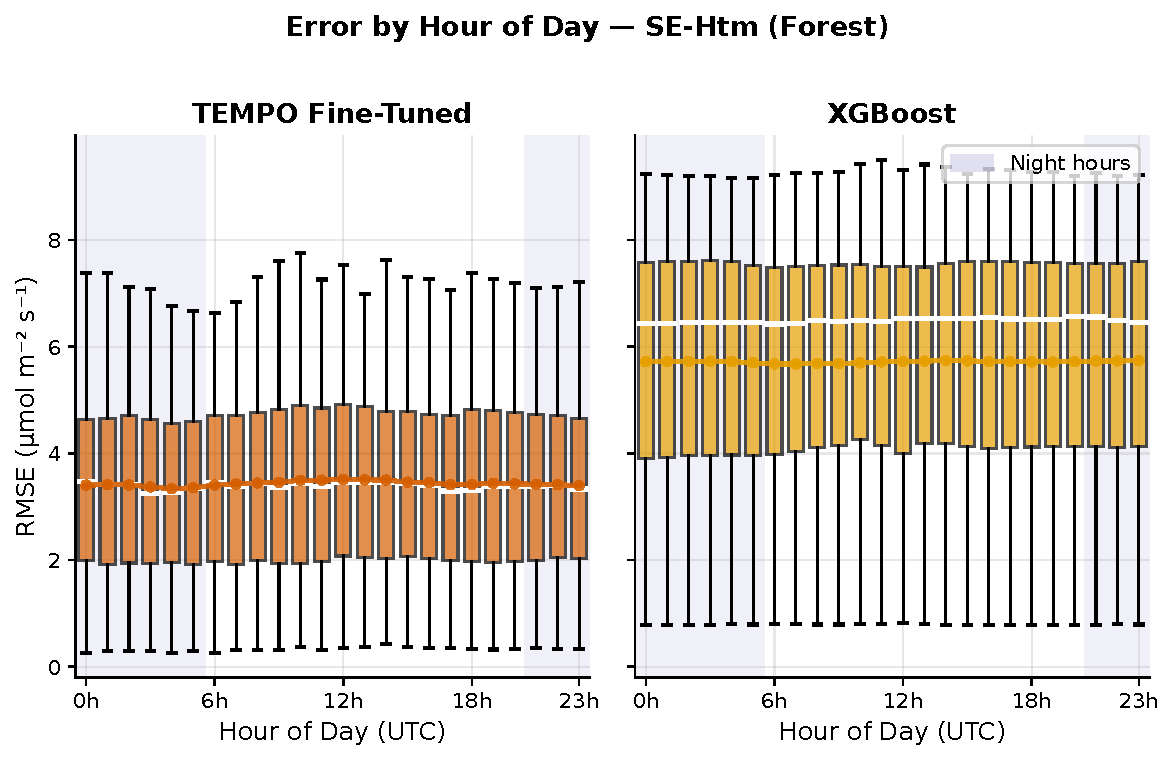
\includegraphics[width=0.95\columnwidth]{figures/error_by_hour_SE-Htm.pdf}
  \Description{Four box-plot panels of forecast RMSE against hour of day, in two
  rows. Top row: the wetland site UK-AMo, with fine-tuned TEMPO (left) and Random
  Forest (right). Bottom row: the forest site SE-Htm, with fine-tuned TEMPO (left)
  and XGBoost (right). The forest error follows a daily oscillation that tracks the
  day--night cycle, whereas the wetland error is flatter and noisier with no clear
  diurnal shape.}
  \caption{Forecast error by hour of day, showing fine-tuned TEMPO against each
  site's strongest baseline (Random Forest for the wetland UK-AMo, top; XGBoost
  for the forest SE-Htm, bottom). The forest shows a regular diurnal error
  pattern; the wetland error is flatter and less structured.}
  \label{fig:errorhour}
\end{figure}

\subsection{Negative transfer across configurations}
\label{sec:negtransfer}
% Source: results/transfer_learning/transfer_matrix.csv,
%         TRANSFER_LEARNING_SUMMARY.txt (negative-transfer cases)
This subsection uses a separate, matched-subsample transfer protocol: each configuration trains on a fixed
$5{,}000$-sample budget so that coverage and leave-one-site-out effects are
compared on equal footing. Baseline $R^2$ under this protocol therefore differ
slightly from the full-test benchmark of Section~\ref{sec:benchmark}; the
results below are read only within this protocol. Sweeping training-data
coverage ($20$--$100\%$) and leave-one-site-out removals over the three
baselines, $33$ of $60$ model--configuration--site combinations ($55\%$)
exhibit negative transfer, where adding source data \emph{harms} target
performance relative to the full-data reference. The
effect is most severe under low coverage on the wetland site (e.g.\ Random
Forest at $20\%$ data, $\Delta R^2 = -0.72$) and recurs in leave-one-site-out
removals (e.g.\ excluding DE-Akm costs Random Forest $\Delta R^2=-0.20$ on
UK-AMo). This is the conventional failure mode the foundation model avoids,
and it reinforces the contrast drawn in Section~\ref{sec:inversion}.
Figure~\ref{fig:transfermatrix} visualises the full transfer matrix under this
matched-subsample protocol.

\begin{figure}[t]
  \centering
  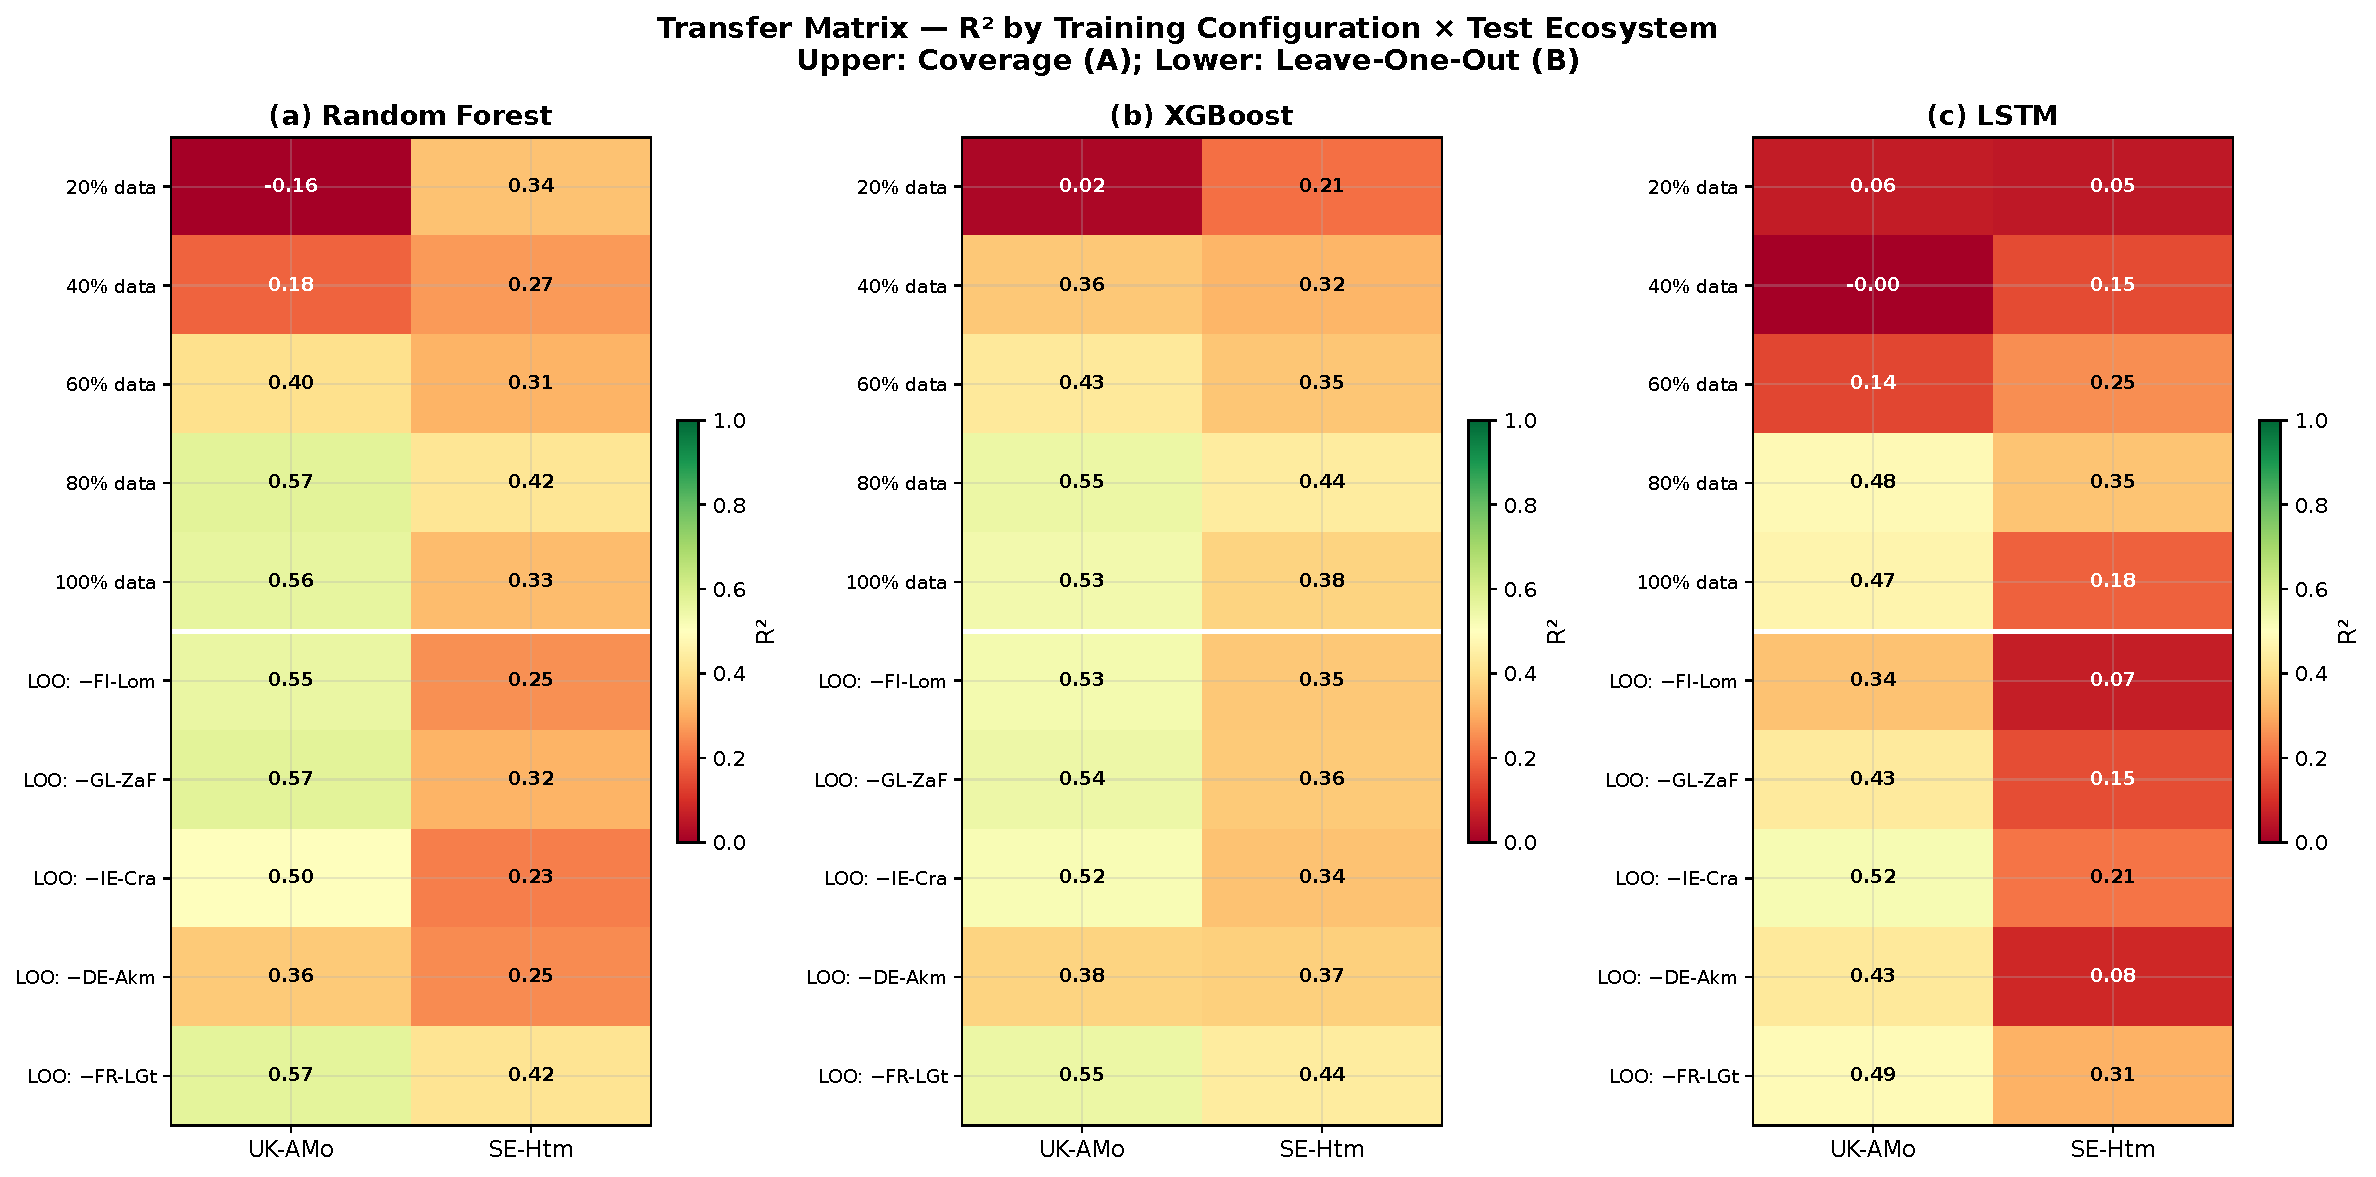
\includegraphics[width=\columnwidth]{figures/transfer_matrix_heatmap.pdf}
  \Description{A three-panel heatmap, one panel per baseline (Random Forest,
  XGBoost, LSTM), with rows for training-coverage and leave-one-site-out
  configurations and columns for the two test sites, cells coloured by
  R-squared. Forest-site columns are consistently darker (lower) than
  wetland-site columns, and low-coverage cells are darkest, marking
  negative-transfer cases.}
  % Source: results/transfer_learning/transfer_matrix.csv (RF 20%-coverage,
  % UK-AMo R2=-0.163); negative_transfer_summary.csv
  \caption{Transfer matrix for the three baselines (Random Forest, XGBoost,
  LSTM) under the matched-subsample protocol of Section~\ref{sec:negtransfer}.
  All three lose skill moving from the wetland to the forest site, and several
  cells show outright negative transfer, e.g.\ Random Forest at $20\%$
  coverage reaches $R^2=-0.16$ on UK-AMo. Baseline values use the
  $5{,}000$-sample protocol and so differ from Table~\ref{tab:penalty}.}
  \label{fig:transfermatrix}
\end{figure}

\subsection{Forecast-horizon analysis}
\label{sec:horizon}
% Source: results/horizon_analysis/horizon_metrics.csv,
%         HORIZON_ANALYSIS_SUMMARY.txt (R2 at key horizons)
A natural objection is that the inversion might be a short-horizon artefact.
It is not. Figure~\ref{fig:horizon} traces $R^2$ across the full $1$--$96$\,h
horizon. On the forest site the foundation model's advantage is stable
throughout: zero-shot TEMPO holds $R^2\approx0.86$ at $1$\,h and still
$R^2=0.742$ at $96$\,h (fine-tuned: $0.886\rightarrow0.681$), while the
baselines start low and decay, XGBoost $0.404\rightarrow0.175$, Random Forest
$0.377\rightarrow0.197$, LSTM $0.338\rightarrow0.151$. The forest gap is
therefore present at every horizon, not just early steps. We are candid about
the wetland site, where the picture is mixed: fine-tuned TEMPO leads at short
horizons ($R^2=0.879$ at $1$\,h) but degrades faster, so by the longest horizon
Random Forest ($R^2=0.487$ at $96$\,h) edges fine-tuned TEMPO ($R^2=0.481$).
The inversion is thus a robust property of the cross-ecosystem forest transfer
across horizons, while same-ecosystem wetland performance is a closer contest.

\begin{figure}[t]
  \centering
  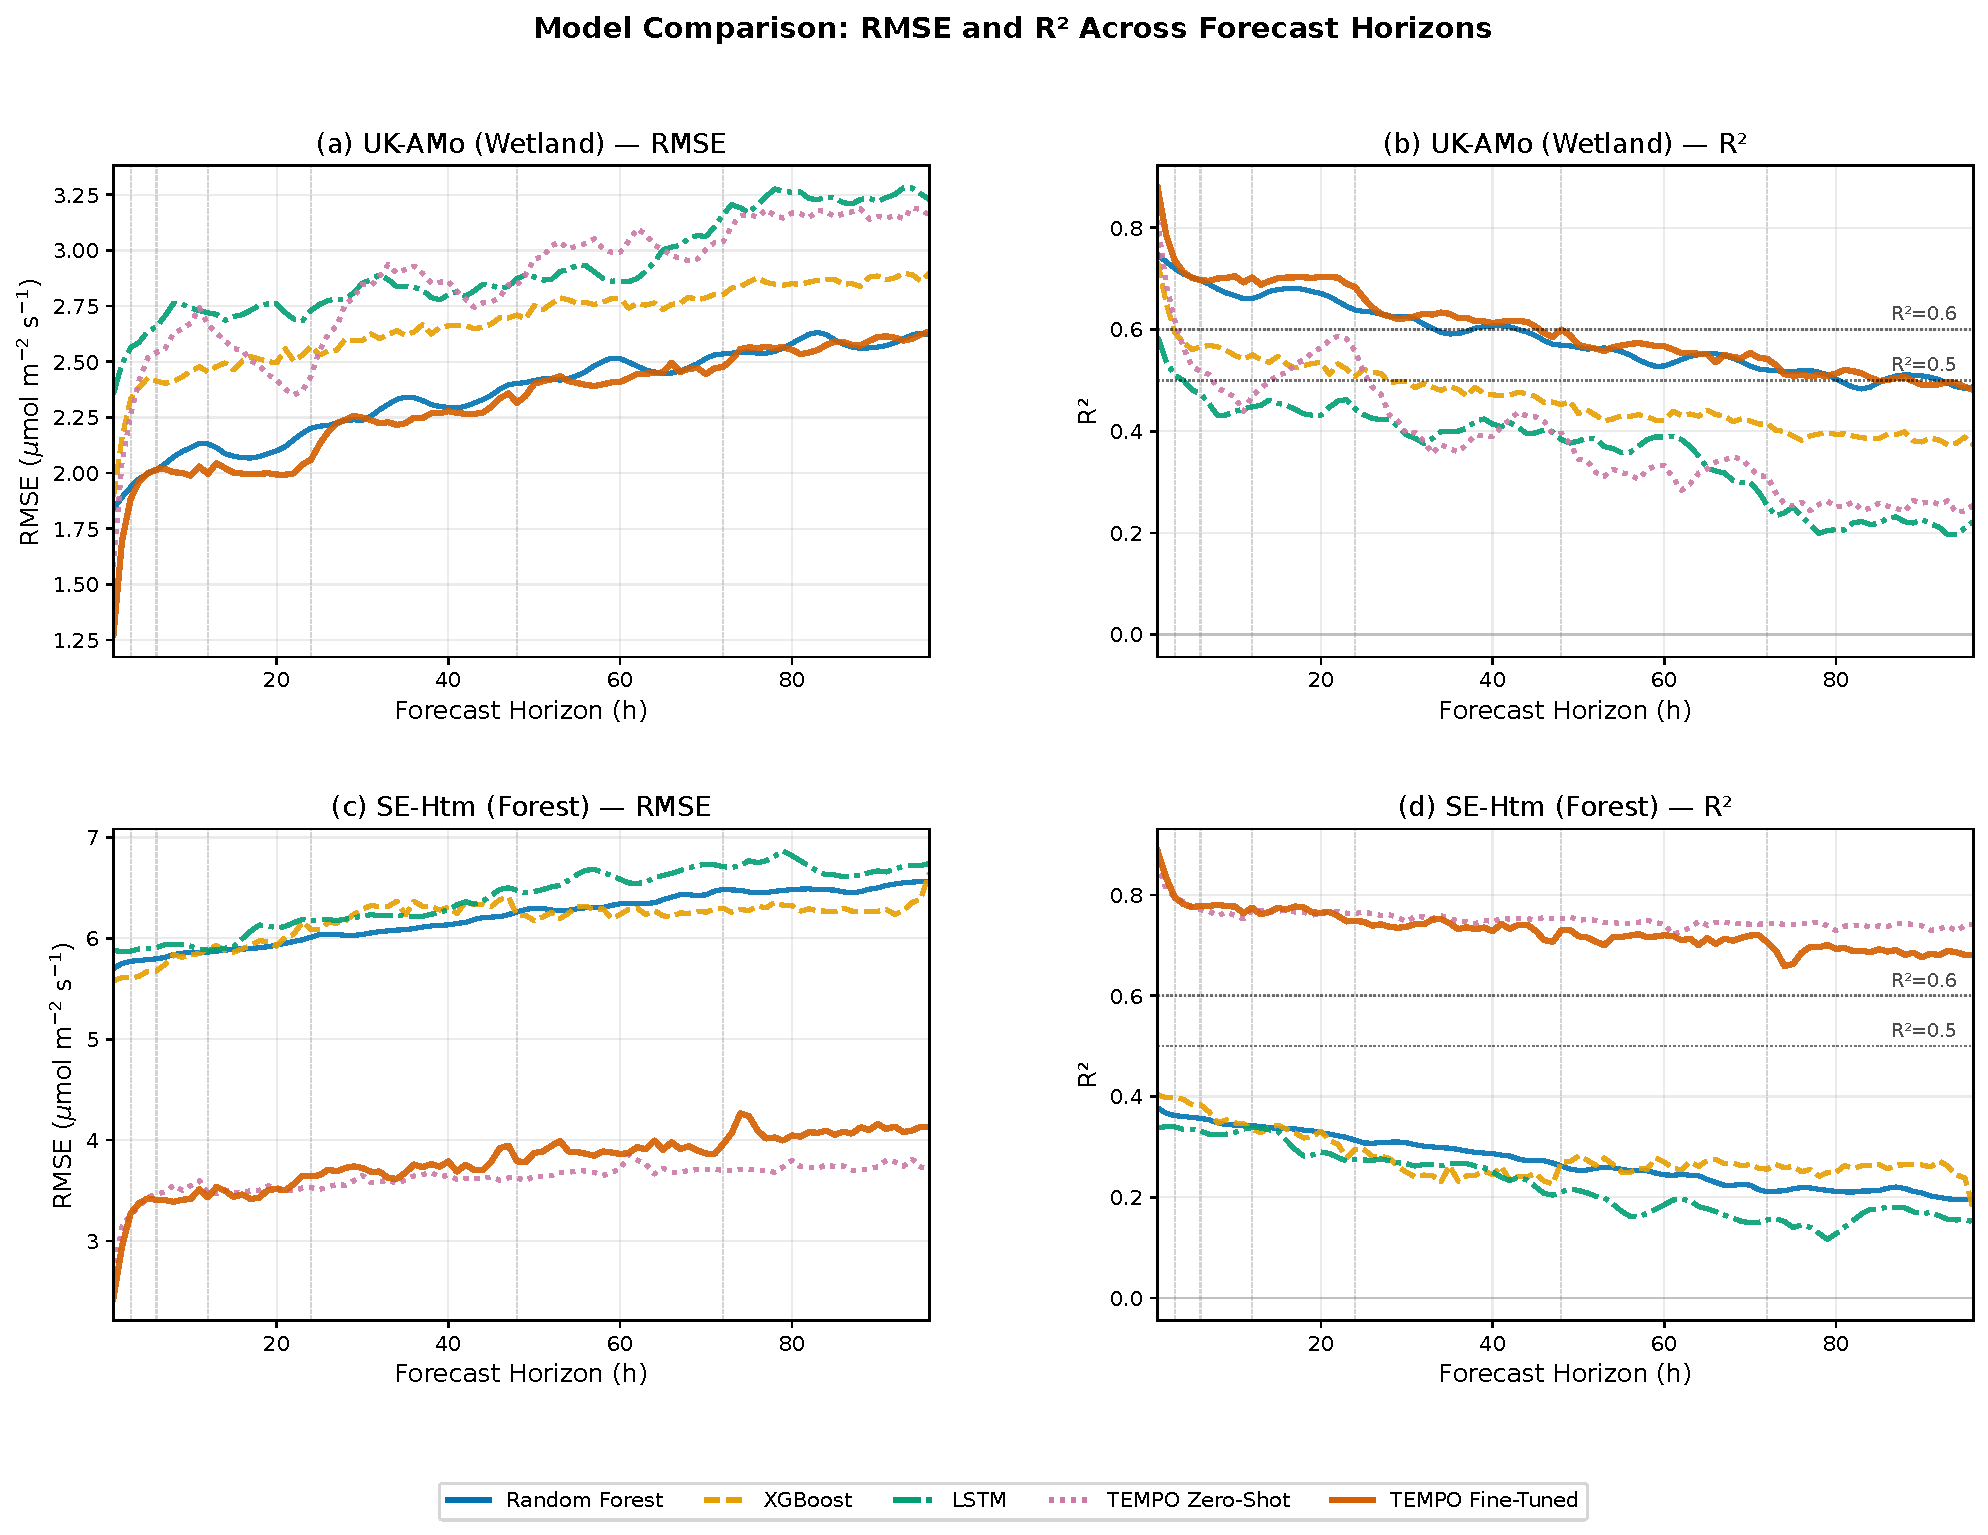
\includegraphics[width=\columnwidth]{figures/model_comparison_by_horizon.pdf}
  \Description{Line plots of R-squared against forecast horizon from 1 to 96
  hours, one line per model, separated by site. On the forest site both TEMPO
  lines stay high and nearly flat while the baseline lines start low and decline;
  on the wetland site TEMPO leads at short horizons but the Random Forest line
  catches up to it by the longest horizon.}
  \caption{$R^2$ versus forecast horizon ($1$--$96$\,h). On the forest site
  (SE-Htm) both TEMPO variants dominate at all horizons; on the wetland site
  (UK-AMo) TEMPO leads early while Random Forest catches up by $96$\,h.}
  \label{fig:horizon}
\end{figure}

\subsection{Statistical significance}
\label{sec:significance}
% Source: results/analysis/pairwise_comparisons.csv
% (cohens_d, p_value_ttest, dm_mdm_statistic for TEMPO Fine-Tuned vs each baseline)
Table~\ref{tab:sig} summarises the pairwise tests of fine-tuned TEMPO against
each baseline on both sites. Every difference is significant at $p<0.001$ under
both a paired $t$-test and the modified Diebold--Mariano (mDM) test on $96$\,h
forecast errors. The effect sizes are revealing: on the wetland site the
effects are small (Cohen's $d$ from $0.14$ vs.\ Random Forest to $0.34$ vs.\
XGBoost), reflecting the close contest there, whereas on the forest site all
three are medium effects ($d=0.53$--$0.55$), confirming the cross-ecosystem
advantage is substantive and not merely significant.

\begin{table}[t]
  \centering
  \caption{Fine-tuned TEMPO vs.\ each baseline: Cohen's $d$, paired $t$-test
  $p$-value, and modified Diebold--Mariano statistic on $96$\,h errors.}
  \label{tab:sig}
  \small
  \begin{tabular}{@{}llccc@{}}
    \toprule
    Site & vs.\ baseline & Cohen's $d$ & $p$ & mDM \\
    \midrule
    \multirow{3}{*}{UK-AMo}
      & Random Forest & 0.140 & $<0.001$ & $-6.50$ \\
      & XGBoost       & 0.337 & $<0.001$ & $-41.66$ \\
      & LSTM          & 0.259 & $<0.001$ & $-43.97$ \\
    \midrule
    \multirow{3}{*}{SE-Htm}
      & XGBoost       & 0.553 & $<0.001$ & $-108.15$ \\
      & Random Forest & 0.534 & $<0.001$ & $-105.31$ \\
      & LSTM          & 0.553 & $<0.001$ & $-79.26$ \\
    \bottomrule
  \end{tabular}
\end{table}

\subsection{Computational cost}
\label{sec:cost}
% Source: results/metrics/computational_costs.json,
%         results/efficiency/efficiency_comparison.csv (baselines only;
%         TEMPO was not profiled in this CPU harness)
Table~\ref{tab:cost} reports the cost of the three baselines from the CPU
efficiency benchmark. All three are cheap and real-time capable: training
ranges from $0.09$\,h (XGBoost) to $1.11$\,h (LSTM), single-sample inference
stays at $3$--$14$\,ms, and peak memory is at most $116$\,MB. The accuracy--cost
trade-off is stark on the forest site, where these inexpensive models reach
only $R^2\le0.28$ (Table~\ref{tab:benchmark}) while the $80$M-parameter
foundation model exceeds $R^2=0.72$. TEMPO's own runtime was not measured in
this CPU harness, so we do not report it; the comparison establishes that the
baselines' speed advantage does not translate into competitive cross-ecosystem
accuracy.

\begin{table}[t]
  \centering
  \caption{Baseline computational cost from the CPU efficiency benchmark.
  Train time, single-sample inference latency, and peak memory.}
  \label{tab:cost}
  \small
  \begin{tabular}{@{}lccc@{}}
    \toprule
    Model & Train (h) & Infer (ms) & Peak mem (MB) \\
    \midrule
    Random Forest & 0.79 & 13.81 & 3.8 \\
    XGBoost       & 0.09 & 3.19  & 0.7 \\
    LSTM          & 1.11 & 6.75  & 116.0 \\
    \bottomrule
  \end{tabular}
\end{table}

% =====================================================================
\section{Discussion}
% =====================================================================

\paragraph{Implications.}
The inverted penalty suggests that foundation models can behave
counter-intuitively in the geosciences. Where classical theory anchors
performance to source--target domain match, a pretrained model's skill appears
to track alignment with its \emph{pretraining} distribution. On the two
held-out sites, the better-forecast forest is distinguished from the wetland
not by a more \emph{regular} signal but by a far larger one: objective measures
show it is, if anything, marginally less regular (higher spectral entropy, lower
lag-24\,h autocorrelation; Table~\ref{tab:regularity}), yet its diurnal cycle is
several times larger in amplitude. The better-supported reading is therefore one
of amplitude and signal-to-noise, a large-amplitude, high-SNR periodic signal
can be forecast more accurately than a suppressed, low-amplitude one even when
the latter is nominally closer to the training biome. We flag honestly that the
normalised regularity measures did \emph{not} support the original ``more
regular'' hypothesis, and that this amplitude reading is inferred from limited
evidence: per-site zero-shot $R^2$ exists for only the two test sites, and
amplitude is not a strict ecosystem property (the wetland DE-Akm has the
second-largest diurnal amplitude of the seven sites). We therefore present it as
the more consistent interpretation rather than a settled mechanism.
For practitioners assembling NEE forecasting systems across sparse tower
networks, this implies that foundation models may generalise to
under-represented but well-behaved ecosystems better than transfer theory
would predict.

\paragraph{Limitations.}
Three caveats bound the claim. First, the \emph{information asymmetry}: the
baselines use $19$ covariates while TEMPO is univariate, so the comparison is
not input-matched; the foundation model's advantage on the forest site is
achieved with strictly less information, but the asymmetry must be named, not
hidden. Second, we evaluate a \emph{single} foundation model. Third, the
inversion is demonstrated on \emph{two} held-out test sites; the direction of
the effect is clear and statistically strong, but its breadth across biomes
remains to be established.

\paragraph{Outlook.}
A natural next step is to remove the information asymmetry by conditioning the
foundation model on the same covariates available to the baselines, and to
broaden the evaluation to additional ecosystems and a global pool of sites.
We leave these extensions to future work.

% =====================================================================
\section{Conclusion}
% =====================================================================

Across contrasting FLUXNET ecosystems, conventional NEE forecasters pay the
classical cross-ecosystem transfer penalty, degrading by $37$--$54\%$ in
$R^2$ performance when moving from a same-biome wetland site to a different 
forest site. Conversely, the pretrained TEMPO foundation model completely 
inverts this behaviour, forecasting the forest target ($R^2=0.728$) with higher 
accuracy than the wetland baseline ($R^2=0.599$). This finding indicates that 
distributional alignment with a foundation model's pretraining corpus can 
outweigh a nominal ecosystem match. Future work will equalise model inputs 
via covariate conditioning and evaluate this inversion across a broader suite 
of global biomes.

% =====================================================================
\begin{acks}
We thank Po Yang for supervision; the FLUXNET community and individual site
principal investigators for maintaining the open FLUXNET2015 database; the
ICOS network; and the developers of TEMPO for releasing the model weights.
%% AI-use disclosure: add a proportional disclosure here if any text, figures
%% or code newly created for this paper were AI-generated, per ACM policy.
%% Editing or polishing the authors' own writing requires no disclosure.
\end{acks}

\bibliographystyle{ACM-Reference-Format}
\bibliography{references}

\end{document}
